\documentclass[paper=a4, fontsize=11pt, frenchb, englishb]{article}

\usepackage{graphicx}
\usepackage{caption}

\renewcommand{\listfigurename}{Liste des images}

\author{Franc Zobo Nomo \and Mohand Said Abdelli}
\title{Rapport sur le TP 5 noté}
\date{\today}

\begin{document}
	\maketitle
	\tableofcontents
	
	\section{Introduction}
	
Ce projet est le travail demander pour le 1er TP noté du cours de programmation objet avancée. On s’intéresse à la gestion de projets qui se décomposent en tâches dépendantes les unes des autres. Suite à la première lecture du TP. Nous avons réaliser le diagramme UML suivant:

\begin{center}
	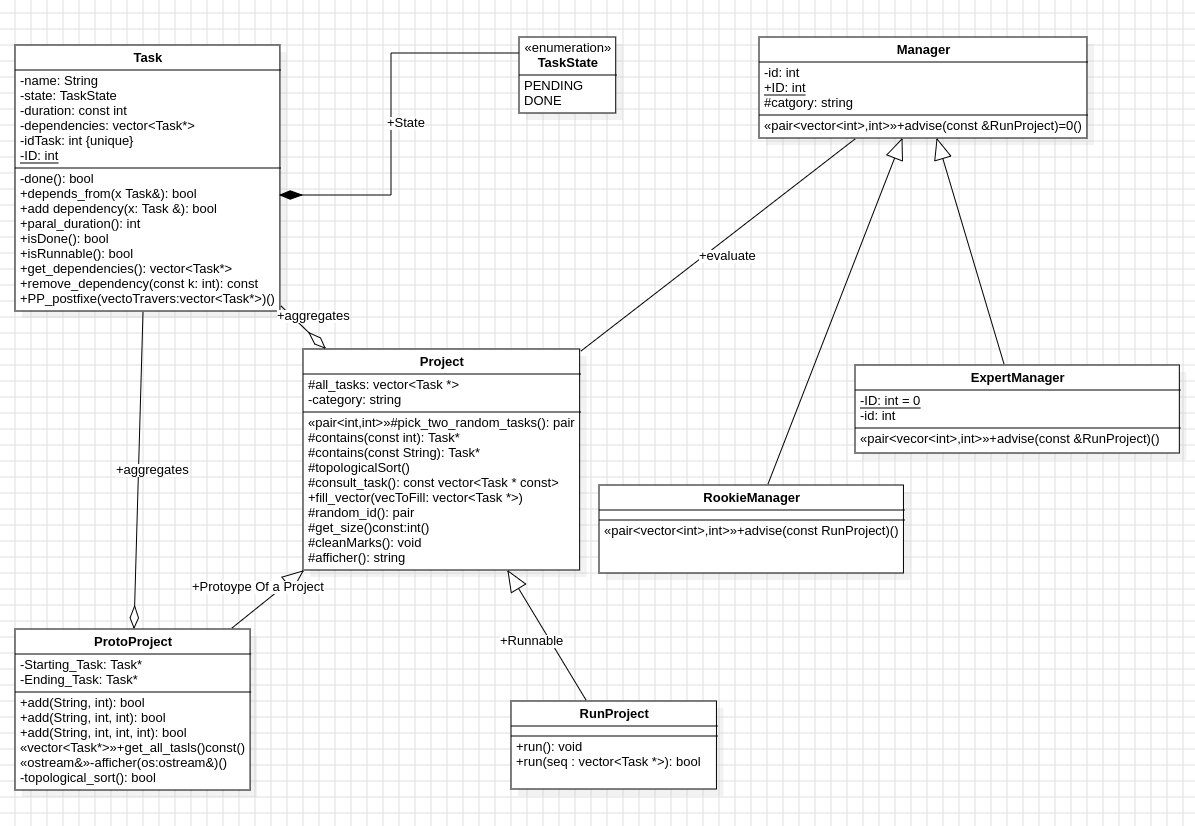
\includegraphics[width=\linewidth]{diagramme-uml.png}
	\captionof{figure}{Diagramme UML}\label{diag}
\end{center}
	
	\section{Code source}
	
		\subsection{Arborescence}
		
Le code source du projet se trouve dans le répertoire src/ qui lui même est composé de 4 sous - répertoire:

\begin{itemize}
	\item header/: Contient tous les fichiers d'en-tête du projet
	\item libs/: Contient les classes annexes servant aux classes principales et classes de tests du projet
	\item main/: Contient les classe principale du projet
	\item test/: Contient les classes de Tests du projet
\end{itemize}

À la racine du projet, on retrouvera un Makefile servant à la compilation, un fichier binôme.md contenant la liste des membres du projet, un README.md reprennant sommairement les éléments de ce rapport et un répertoire docs/ où l'on pourra retrouver le diagramme UML ainsi que ce rapport.
		
		\subsection{Partie Tâche}
		
			\paragraph{bool done()}
			
On change le statut (on le passe à DONE) de la tache et retourne vrai si toute ses dépendance ont le statut DONE. sinon on retourne faux.
			
			\paragraph{bool depends\_from(Task)}
Cette fonction est récursive. On retourne faux si la dépendance est vide ou si la tache passé en paramètre n'appartient pas à la liste de dépendance de notre tache, ni à aucune sous dépendance (l'appel à depends\_from sous chaque dépendance doit retourner faux). Sinon retourne vrai.

			\paragraph{bool add\_dependency(Task)}
			
Retourne vrai si la tache penser en argument ne dépends pas de notre tache et que l'ajout de la tache passer en argument à la liste de dépendance de notre tache ne pose pas problème. Sinon retourne faux.
			
			\paragraph{bool paral\_duration()}
			
Cette fonction est récursive. On retourne la durée de la tache ajoute au max de paral\_duration() de toute ses dépendances.

			\paragraph{PP\_postfixe()}
			
Le tri topologique de la classe Project dépends de cette méthode de Task. Elle vérifie si la tâche appelante n'est pas marqué (if (!this-$>$mark)). si elle n'est pas encore 
marqué, elle vérifie si chacunes de ses dépendances est marquée en faisant un appelle recursif dans ine foucle for sur les vecteurs de dépendances. À la fin elle fait un 
push\_back(this);

		
		\subsection{Partie Projet}
		
			\subsubsection{Project}
			
				\paragraph{Pick\_two\_random\_task()}
				
Prends deux indice retourné par random\_id() et cherche les id de chacun des indices dans le vecteur de tache, récupére leur pointeur. Ensuite elle verifie si les deux tache 
sélectionné sont compatibles en terme de dépendance. Si elle sont dépendantes elle réitère ( 50 fois la taille du vecteur de tache). Elle retourne la valeur des deux id à
la fin.

				\paragraph{topological\_sort()}
				
\begin{itemize}
	\item Crée un vecteur de pointeur de Task.
	\item Fait clearMarks() pour l'objet qui appelé. 
	\item Fait appel à la méthode PP\_postfixe() sur l'objet pointé par this->all\_tasks[0]
	\item Qui prend en argument la référence du vecteur crée et remplit par les valeurs des pointeur des taches de l'objet appelant. 
	\item Vérifie si la taille de vecteur passé en référence a une taille égal au vecteur vecteurs de pointeur de tache de l'objet appelant pour savoir si le tri topologique a été
	possible. 
	\item Elle si c'est le cas, elle remplit le vecteur de pointeur de tache de l'objet appelant par les valeurs du vecteur passer par référence pour PP\_postfixe et retourne vrai.
	Sinon elle retourne faux.
	
\end{itemize}

			\subsubsection{ProtoProject}
			
				\paragraph{bool add(const string, const int)}
				
Cette méthode prend en argument un string pour le nom de task et une duration pour créé dynamique une tache avec ces arguments. ensuite elle execute une boucle ou elle 
vérifie la dépenedance de deux taches sélectionné au hasard en utilisant la méthode de Project random\_id qui retourne une pair<int,int> de deux id des taches contenue dans 
le vecteur all\_tasks. Elle récupère les pointeurs, vérifie ensuite que les deux taches avec les ids correspendant existe dans le vecteur de taches et si t ne dépends pas de 
de t2(le cas favorable à l'ajout), elle ajoute donc t1 aux dépendances de la tâche créer et ajoute la nouvelle tache créer au dépendance de t2 et fait le tri topologique 
qui retourne aussi une valeur booléenne témoignant le succès de l'ajout et la satisfaction d'un DAG. dans le cas où t1 dépends de t2 ou que le tri topologique échoue, la 
nouvelle taches est supprimé, et son pointeur est aussi supprimer du vecteur de dépendances de chaque tâches du vecteur de pointeur de tache de ProtoProject, et on boucle 
jusqu'à ce qu'on tombe sur des IDs qui satisfait la condition.

				
				\paragraph{bool add(const string, const int, const int)}
				
Cette méthode prend en argument un string pour le nom de la tâches, un int pour la duration, un autre int qui est un id d'une tache de laquelle la nouvelle tâches qu'on va 
créer doit dépendre. on prend alors l'id, on vérifie qu'il est correcte et on récupère le pointeur vers cette tâches. on ajoute ensuite la nouvelle tâches au dépendance de 
fin, on rajoute à la taches qu'on a créer sa dépendances à la taches t. on fait le tri topologique. si le tri retourne vrai, on retourne vrai, sinon on supprime la nouvelle 
taches, et on supprime son pointeur des dépendance de toutes les tâches du vecteurs all\_tasks de ProtoProject et retourne faux.

				
				\paragraph{bool add(const string, const int, const int, const int)}
				
Cette méthode prends un nom pour une nouvelle taĉhes, sa duration, deux id de tâches *t\_avn et *t\_apn. on utilise les ids pour récupérer les tâches si elle existe. on 
verifie ensuite la dépendance de t1 à t2 et place la nouvelle tâches en utilisant la même approches de vérification de dépendance entre t\_avn et t\_apn que l'approches 
utilser pour l'ajout d'une taches entre deux taches aléatoire sauf que dans le cas actuel, on fait les test sur les tache t\_avs et t\_apn.

			
			\subsubsection{RunProject}
			
				\paragraph{int run(const int)}
				
Cette méthodes vérifie si toutes les dépendances de la tâches de l'id reçu en argument sont exécuté, si c'est le cas elle execute la tache en question sinon elle retourne 
faux.
				
				\paragraph{int run(const vector $<$int$>$)}
				
Cette méthode vérifie la possibilité de l'execution de chaque taches avant de passé à la suivante. si elle trouve qu'une tâches ne peut pas être exécuter car ses 
dépendances ne sont pas exécuté, elle retourne faux.

		
		\subsection{Partie Gestionnaire}
		
			\subsubsection{RookieManager}
			
				\paragraph{pair$<$vector$<$int$>$, int$>$ avis(const RunProjet)}
				
Les taches du RunProject sont triée de manière topologique donc le premier élément de la pair à retourné contient la liste de tous les id des taches non effectués du vecteurs all\_tasks dans l'ordre inverse. Le deuxième élément de la pair est simplement la somme de toute les taches ayant un id dans le premier élément de la pair.
			
			\subsubsection{ExpertManager}
			
				\paragraph{pair$<$vector$<$int$>$, int$>$ avis(const RunProjet)}
				
Les taches sont arrangé sur plusieurs niveau selon leurs niveau de dépendances. Le niveau 0, ne contient que la tache de fin. Plus le niveau est au moins la tache contient de dépendances. Dans le premier élément de la pair on empile les éléments de la pair allant du plus haut niveau au niveau 0. Le second élément de la pair est simplement soit -1 si le premier élement de la pair est une liste vide ou le résultat de la fonction paral\_duration() sur la dernière tâche ajouter dans le premier élément de la pair.
	
	\section{Compilation}
	
		\subsection{Les commandes de compilation}
		
La compilation peut se faire par deux moyens différents soit en effectuant la commande:

\begin{itemize}
	\item make: qui crée tout les répertoire nécessaire et compilera tout les fichiers tu projet pour pouvoir réaliser les tests.
	\item make TestNomdeClasse: (remplacer NomdeClasse par le nom d'une classe sauf Manager et Project) la commande compilera tout les fichiers nécessaire pour pouvoir tester cette Classe.
\end{itemize}
		
		\subsection{Le rendu de compilation}
		
Les commandes de compilation créeront trois répertoires:

\begin{itemize}
	\item bin/ : contenant les fichiers compilés à exécuter
	\item bin/obj : contenant les fichier objet servant à construire les fichiers exécutable
	\item log/ : contenant la trace de l' exécution de nos programme
\end{itemize}
	
	\section{Les tests}
	
Les commandes de compilation résulteront la création de fichiers tests permettant de tester les classes principale du projets.\\

\noindent Liste des fichiers sont les suivant:

\begin{itemize}
	\item ./bin/TestTask
	\item ./bin/TestProtoProject
	\item ./bin/TestRunProject
	\item ./bin/TestRookieManager
	\item ./bin/TestExpertManager
\end{itemize}

Les Tests sont indépendant entre la partie Projet et la partie Gestionnaire. On supposera que les fonctions situé dans la partie Projet ou Gestionnaire nous renverra les bonnes valeurs pour qu'on puisse uniquement Tester la partie que l'on souhaite.\\

\noindent Les tests ont été effectuer en tenant compte des diagrammes suivant:

\begin{center}
	\includegraphics[width=0.2\linewidth]{assets/t1.png}
	\captionof{figure}{Arborescence de tâche minimal}\label{t1}
\end{center}

\begin{center}
	\includegraphics[width=0.6\linewidth]{assets/t2.png}
	\captionof{figure}{Arborescence de tâche simple}\label{t2}
\end{center}

\begin{center}
	\includegraphics[width=0.7\linewidth]{assets/t3.png}
	\captionof{figure}{Arborescence de tâche construit}\label{t3}
\end{center}

\begin{center}
	\includegraphics[width=\linewidth]{assets/t4.png}
	\captionof{figure}{Arborescence de tâche élaboré}\label{t4}
\end{center}

\noindent Pour lancer tout tester les parties du projet deux moyens s'impose à vous:

\begin{itemize}
	\item Lancer la commande : make test\_All. 
	\item Lancer la commande : make test\_Nomdelaclasse.
\end{itemize}
	
		\subsection{Tester la partie Tâche}
		
Dans cette section se sont les fonctions done(), add\_dependency(Task t) et paral\_duration() qui seront tester. On teste si les fonctions effectuent bien l'action souhaiter afficher à la fin du test puis on affichera le résultat du test succeed ou failed. Le code source se trouve dans la classe TestTask.cpp.
		
		\subsection{Tester la partie Projet}
	
Dans cette section se sont les classes ProtoProject et RunProject qui sont tester.\\
	
\noindent Pour la classe ProtoProject, se sont les fonctions topological\_sot(); sur le shéma \ref{t3} et \ref{t4} et les trois méthode add() qui seront tester. On teste si les fonctions effectuent bien l'action souhaiter afficher à la fin du test puis on affichera le résultat du test succeed ou failed. Le code source se trouve dans la classe TestProtoProject.cpp.\\

\noindent Pour la classe RunProject, se sont les fonctions 2 run(); sur le shéma \ref{t4} qui seront tester. On teste si les fonctions effectuent bien l'action souhaiter afficher à la fin du test puis on affichera le résultat du test succeed ou failed. Le code source se trouve dans la classe TestRunProject.cpp.
		
		\subsection{Tester la partie Gestionnaire}
		
Dans cette section se sont les classes RookieManager et ExpertManager qui sont tester.\\

\noindent Pour la classe RookieManager, c'est la fonction avis() sur le shéma de \ref{t1} à \ref{t4}  qui est tester. On teste si la fonction effectuent bien l'action souhaiter afficher à la fin du test puis on affichera le résultat du test succeed ou failed. Le code source se trouve dans la classe TestRookieManager.cpp.\\

\noindent Pour la classe ExpertManager,  c'est la fonction avis() sur le shéma de \ref{t1} à \ref{t4}  qui est tester. On teste si la fonction effectuent bien l'action souhaiter afficher à la fin du test puis on affichera le résultat du test succeed ou failed. Le code source se trouve dans la classe TestExpertManager.cpp.
	
	\section{À ajouter}
	
		\subsection{Les ressenties}
		
Nous avons plutôt apprécier ce TP, Il n'a pas été très difficile à réaliser les seules difficultés que nous avons rencontré ont été le manque de précisions sur certaines partie du sujet ainsi que la modélisation UML du concept.
		
		\subsection{Remerciements}
		
Nous remercions notre enseignant JURSKI Yan qui nous aidé à réaliser le TP en présentiel le 24 octobre et qui a répondu à nombreuse de nos questions par courriel.

\newpage
\listoffigures
	

\end{document}